% Options for packages loaded elsewhere
\PassOptionsToPackage{unicode}{hyperref}
\PassOptionsToPackage{hyphens}{url}
\PassOptionsToPackage{dvipsnames,svgnames,x11names}{xcolor}
%
\documentclass[
  letterpaper,
  DIV=11,
  numbers=noendperiod]{scrreprt}

\usepackage{amsmath,amssymb}
\usepackage{lmodern}
\usepackage{iftex}
\ifPDFTeX
  \usepackage[T1]{fontenc}
  \usepackage[utf8]{inputenc}
  \usepackage{textcomp} % provide euro and other symbols
\else % if luatex or xetex
  \usepackage{unicode-math}
  \defaultfontfeatures{Scale=MatchLowercase}
  \defaultfontfeatures[\rmfamily]{Ligatures=TeX,Scale=1}
\fi
% Use upquote if available, for straight quotes in verbatim environments
\IfFileExists{upquote.sty}{\usepackage{upquote}}{}
\IfFileExists{microtype.sty}{% use microtype if available
  \usepackage[]{microtype}
  \UseMicrotypeSet[protrusion]{basicmath} % disable protrusion for tt fonts
}{}
\makeatletter
\@ifundefined{KOMAClassName}{% if non-KOMA class
  \IfFileExists{parskip.sty}{%
    \usepackage{parskip}
  }{% else
    \setlength{\parindent}{0pt}
    \setlength{\parskip}{6pt plus 2pt minus 1pt}}
}{% if KOMA class
  \KOMAoptions{parskip=half}}
\makeatother
\usepackage{xcolor}
\setlength{\emergencystretch}{3em} % prevent overfull lines
\setcounter{secnumdepth}{5}
% Make \paragraph and \subparagraph free-standing
\ifx\paragraph\undefined\else
  \let\oldparagraph\paragraph
  \renewcommand{\paragraph}[1]{\oldparagraph{#1}\mbox{}}
\fi
\ifx\subparagraph\undefined\else
  \let\oldsubparagraph\subparagraph
  \renewcommand{\subparagraph}[1]{\oldsubparagraph{#1}\mbox{}}
\fi

\usepackage{color}
\usepackage{fancyvrb}
\newcommand{\VerbBar}{|}
\newcommand{\VERB}{\Verb[commandchars=\\\{\}]}
\DefineVerbatimEnvironment{Highlighting}{Verbatim}{commandchars=\\\{\}}
% Add ',fontsize=\small' for more characters per line
\usepackage{framed}
\definecolor{shadecolor}{RGB}{241,243,245}
\newenvironment{Shaded}{\begin{snugshade}}{\end{snugshade}}
\newcommand{\AlertTok}[1]{\textcolor[rgb]{0.68,0.00,0.00}{#1}}
\newcommand{\AnnotationTok}[1]{\textcolor[rgb]{0.37,0.37,0.37}{#1}}
\newcommand{\AttributeTok}[1]{\textcolor[rgb]{0.40,0.45,0.13}{#1}}
\newcommand{\BaseNTok}[1]{\textcolor[rgb]{0.68,0.00,0.00}{#1}}
\newcommand{\BuiltInTok}[1]{\textcolor[rgb]{0.00,0.23,0.31}{#1}}
\newcommand{\CharTok}[1]{\textcolor[rgb]{0.13,0.47,0.30}{#1}}
\newcommand{\CommentTok}[1]{\textcolor[rgb]{0.37,0.37,0.37}{#1}}
\newcommand{\CommentVarTok}[1]{\textcolor[rgb]{0.37,0.37,0.37}{\textit{#1}}}
\newcommand{\ConstantTok}[1]{\textcolor[rgb]{0.56,0.35,0.01}{#1}}
\newcommand{\ControlFlowTok}[1]{\textcolor[rgb]{0.00,0.23,0.31}{#1}}
\newcommand{\DataTypeTok}[1]{\textcolor[rgb]{0.68,0.00,0.00}{#1}}
\newcommand{\DecValTok}[1]{\textcolor[rgb]{0.68,0.00,0.00}{#1}}
\newcommand{\DocumentationTok}[1]{\textcolor[rgb]{0.37,0.37,0.37}{\textit{#1}}}
\newcommand{\ErrorTok}[1]{\textcolor[rgb]{0.68,0.00,0.00}{#1}}
\newcommand{\ExtensionTok}[1]{\textcolor[rgb]{0.00,0.23,0.31}{#1}}
\newcommand{\FloatTok}[1]{\textcolor[rgb]{0.68,0.00,0.00}{#1}}
\newcommand{\FunctionTok}[1]{\textcolor[rgb]{0.28,0.35,0.67}{#1}}
\newcommand{\ImportTok}[1]{\textcolor[rgb]{0.00,0.46,0.62}{#1}}
\newcommand{\InformationTok}[1]{\textcolor[rgb]{0.37,0.37,0.37}{#1}}
\newcommand{\KeywordTok}[1]{\textcolor[rgb]{0.00,0.23,0.31}{#1}}
\newcommand{\NormalTok}[1]{\textcolor[rgb]{0.00,0.23,0.31}{#1}}
\newcommand{\OperatorTok}[1]{\textcolor[rgb]{0.37,0.37,0.37}{#1}}
\newcommand{\OtherTok}[1]{\textcolor[rgb]{0.00,0.23,0.31}{#1}}
\newcommand{\PreprocessorTok}[1]{\textcolor[rgb]{0.68,0.00,0.00}{#1}}
\newcommand{\RegionMarkerTok}[1]{\textcolor[rgb]{0.00,0.23,0.31}{#1}}
\newcommand{\SpecialCharTok}[1]{\textcolor[rgb]{0.37,0.37,0.37}{#1}}
\newcommand{\SpecialStringTok}[1]{\textcolor[rgb]{0.13,0.47,0.30}{#1}}
\newcommand{\StringTok}[1]{\textcolor[rgb]{0.13,0.47,0.30}{#1}}
\newcommand{\VariableTok}[1]{\textcolor[rgb]{0.07,0.07,0.07}{#1}}
\newcommand{\VerbatimStringTok}[1]{\textcolor[rgb]{0.13,0.47,0.30}{#1}}
\newcommand{\WarningTok}[1]{\textcolor[rgb]{0.37,0.37,0.37}{\textit{#1}}}

\providecommand{\tightlist}{%
  \setlength{\itemsep}{0pt}\setlength{\parskip}{0pt}}\usepackage{longtable,booktabs,array}
\usepackage{calc} % for calculating minipage widths
% Correct order of tables after \paragraph or \subparagraph
\usepackage{etoolbox}
\makeatletter
\patchcmd\longtable{\par}{\if@noskipsec\mbox{}\fi\par}{}{}
\makeatother
% Allow footnotes in longtable head/foot
\IfFileExists{footnotehyper.sty}{\usepackage{footnotehyper}}{\usepackage{footnote}}
\makesavenoteenv{longtable}
\usepackage{graphicx}
\makeatletter
\def\maxwidth{\ifdim\Gin@nat@width>\linewidth\linewidth\else\Gin@nat@width\fi}
\def\maxheight{\ifdim\Gin@nat@height>\textheight\textheight\else\Gin@nat@height\fi}
\makeatother
% Scale images if necessary, so that they will not overflow the page
% margins by default, and it is still possible to overwrite the defaults
% using explicit options in \includegraphics[width, height, ...]{}
\setkeys{Gin}{width=\maxwidth,height=\maxheight,keepaspectratio}
% Set default figure placement to htbp
\makeatletter
\def\fps@figure{htbp}
\makeatother
\newlength{\cslhangindent}
\setlength{\cslhangindent}{1.5em}
\newlength{\csllabelwidth}
\setlength{\csllabelwidth}{3em}
\newlength{\cslentryspacingunit} % times entry-spacing
\setlength{\cslentryspacingunit}{\parskip}
\newenvironment{CSLReferences}[2] % #1 hanging-ident, #2 entry spacing
 {% don't indent paragraphs
  \setlength{\parindent}{0pt}
  % turn on hanging indent if param 1 is 1
  \ifodd #1
  \let\oldpar\par
  \def\par{\hangindent=\cslhangindent\oldpar}
  \fi
  % set entry spacing
  \setlength{\parskip}{#2\cslentryspacingunit}
 }%
 {}
\usepackage{calc}
\newcommand{\CSLBlock}[1]{#1\hfill\break}
\newcommand{\CSLLeftMargin}[1]{\parbox[t]{\csllabelwidth}{#1}}
\newcommand{\CSLRightInline}[1]{\parbox[t]{\linewidth - \csllabelwidth}{#1}\break}
\newcommand{\CSLIndent}[1]{\hspace{\cslhangindent}#1}

\KOMAoption{captions}{tableheading}
\makeatletter
\makeatother
\makeatletter
\@ifpackageloaded{bookmark}{}{\usepackage{bookmark}}
\makeatother
\makeatletter
\@ifpackageloaded{caption}{}{\usepackage{caption}}
\AtBeginDocument{%
\ifdefined\contentsname
  \renewcommand*\contentsname{Table of contents}
\else
  \newcommand\contentsname{Table of contents}
\fi
\ifdefined\listfigurename
  \renewcommand*\listfigurename{List of Figures}
\else
  \newcommand\listfigurename{List of Figures}
\fi
\ifdefined\listtablename
  \renewcommand*\listtablename{List of Tables}
\else
  \newcommand\listtablename{List of Tables}
\fi
\ifdefined\figurename
  \renewcommand*\figurename{Figure}
\else
  \newcommand\figurename{Figure}
\fi
\ifdefined\tablename
  \renewcommand*\tablename{Table}
\else
  \newcommand\tablename{Table}
\fi
}
\@ifpackageloaded{float}{}{\usepackage{float}}
\floatstyle{ruled}
\@ifundefined{c@chapter}{\newfloat{codelisting}{h}{lop}}{\newfloat{codelisting}{h}{lop}[chapter]}
\floatname{codelisting}{Listing}
\newcommand*\listoflistings{\listof{codelisting}{List of Listings}}
\makeatother
\makeatletter
\@ifpackageloaded{caption}{}{\usepackage{caption}}
\@ifpackageloaded{subcaption}{}{\usepackage{subcaption}}
\makeatother
\makeatletter
\@ifpackageloaded{tcolorbox}{}{\usepackage[many]{tcolorbox}}
\makeatother
\makeatletter
\@ifundefined{shadecolor}{\definecolor{shadecolor}{rgb}{.97, .97, .97}}
\makeatother
\makeatletter
\makeatother
\ifLuaTeX
  \usepackage{selnolig}  % disable illegal ligatures
\fi
\IfFileExists{bookmark.sty}{\usepackage{bookmark}}{\usepackage{hyperref}}
\IfFileExists{xurl.sty}{\usepackage{xurl}}{} % add URL line breaks if available
\urlstyle{same} % disable monospaced font for URLs
\hypersetup{
  pdftitle={R guide for Strategic Information Advisors},
  pdfauthor={Lemlem Baraki, Aaron Chafetz, Tim Essam, Baboyma Kagniniwa, Karishma Srikanth},
  colorlinks=true,
  linkcolor={blue},
  filecolor={Maroon},
  citecolor={Blue},
  urlcolor={Blue},
  pdfcreator={LaTeX via pandoc}}

\title{R guide for Strategic Information Advisors}
\author{Lemlem Baraki, Aaron Chafetz, Tim Essam, Baboyma Kagniniwa,
Karishma Srikanth}
\date{8/1/23}

\begin{document}
\maketitle
\ifdefined\Shaded\renewenvironment{Shaded}{\begin{tcolorbox}[breakable, enhanced, frame hidden, interior hidden, sharp corners, boxrule=0pt, borderline west={3pt}{0pt}{shadecolor}]}{\end{tcolorbox}}\fi

\renewcommand*\contentsname{Table of contents}
{
\hypersetup{linkcolor=}
\setcounter{tocdepth}{2}
\tableofcontents
}
\bookmarksetup{startatroot}

\hypertarget{preface}{%
\chapter*{Preface}\label{preface}}
\addcontentsline{toc}{chapter}{Preface}

\markboth{Preface}{Preface}

Welcome to the first edition of
\texttt{R\ Guide\ for\ Strategic\ Information\ Advisers}!

This edition is an initial release of the manual in anticipation of the
PEPFAR/USAID Data Workshop scheduled for later this summer. This manual
will be used as a supporting material for \texttt{R\ Track} sessions
during the workshop as well as regular reference document for new and
current staffing using R as their primary analytics tool.

The main sections of the manual are:

\begin{itemize}
\tightlist
\item
  Guidance on how to install and configure R, RStudio, RTools, base R
  packages, Fonts and git, as well as structure R Projects to support
  reproducibility.
\item
  Best practices on how to access and work with data, write R scripts.
\item
  Resources on how to use GitHub, GitHub Organization, and reprex to
  speedy assistance.
\item
  Documentation on how to develop R Packages and corresponding
  vignettes, create GitHub Pages, and a personal profile.
\item
  Tips and Tricks.
\end{itemize}

\bookmarksetup{startatroot}

\hypertarget{introduction}{%
\chapter{Introduction}\label{introduction}}

This is a book created from markdown and executable code.

See Chafetz (2023) for additional discussion of literate programming.

\bookmarksetup{startatroot}

\hypertarget{summary}{%
\chapter{Summary}\label{summary}}

Summary is forth coming ...

\bookmarksetup{startatroot}

\hypertarget{background}{%
\chapter{Background}\label{background}}

Maintain a standard, living reference guide to establish standard
workflows and for onboard analysts on how to access the great work that
exists and be a contributor as well. See OHA R Analyst Manual -
Purpose/Outline for more details. This guide is not intended to teach
you R, but rather how to orient you to how we have set up and use R
workflows. If you are looking for a getting started with R guide, we
developed a
\href{https://usaid-oha-si.github.io/learn/categories/\#rbbs}{``R
Building Blocks Series''} in 2022 based on
\href{https://r4ds.had.co.nz/}{R for Data Science}.

\hypertarget{who-is-the-audience}{%
\section{Who is the audience?}\label{who-is-the-audience}}

This guide is designed to assist OHA analysts who want to incorporate R
+ RStudio and Git + GitHub into their analytical workflows. While the
primary target audience is new Strategic Information Analysts, the
concepts covered in this guide can be readily applied to workflows
across various areas within OHA.

\hypertarget{how-to-use}{%
\section{How to use}\label{how-to-use}}

This guide is setup to help users setup their R environments on their
local machines

\hypertarget{how-to-contribute}{%
\section{How to contribute}\label{how-to-contribute}}

TO DO

\part{Tools and configurations}

\hypertarget{installing-r-rstudio-rtools}{%
\chapter{Installing R, RStudio,
RTools}\label{installing-r-rstudio-rtools}}

Working from your USAID laptop, Government Furnished Equipment (GFE),
you can install R and RStudio without having to submit a ticket to the
M/CIO Help Desk. R is the open-source statistics package that we use for
our work and is the engine that powers RStudio Desktop, the user
interface or integrated development environment (IDE). RStudio Desktop
or another IDE such as Visual Studio Code is not required to use R, but
will vastly improve your experience.

To install both R and RStudio Desktop on your GFE, go to Software Center
on your computer (Start \textgreater{} Microsoft Endpoint manager
\textgreater{} Software Center) Once there, you can select the
Application called ``R for Windows'' and click ``Install''. After that
completes, you can then select ``RStudio Desktop'' and then ``Install''.
If you run into any issues, first try restarting your machine and if
that fails, you can contact \href{CIO-HELPDESK@usaid.gov}{M/CIO Help
Desk}.

\begin{figure}

{\centering 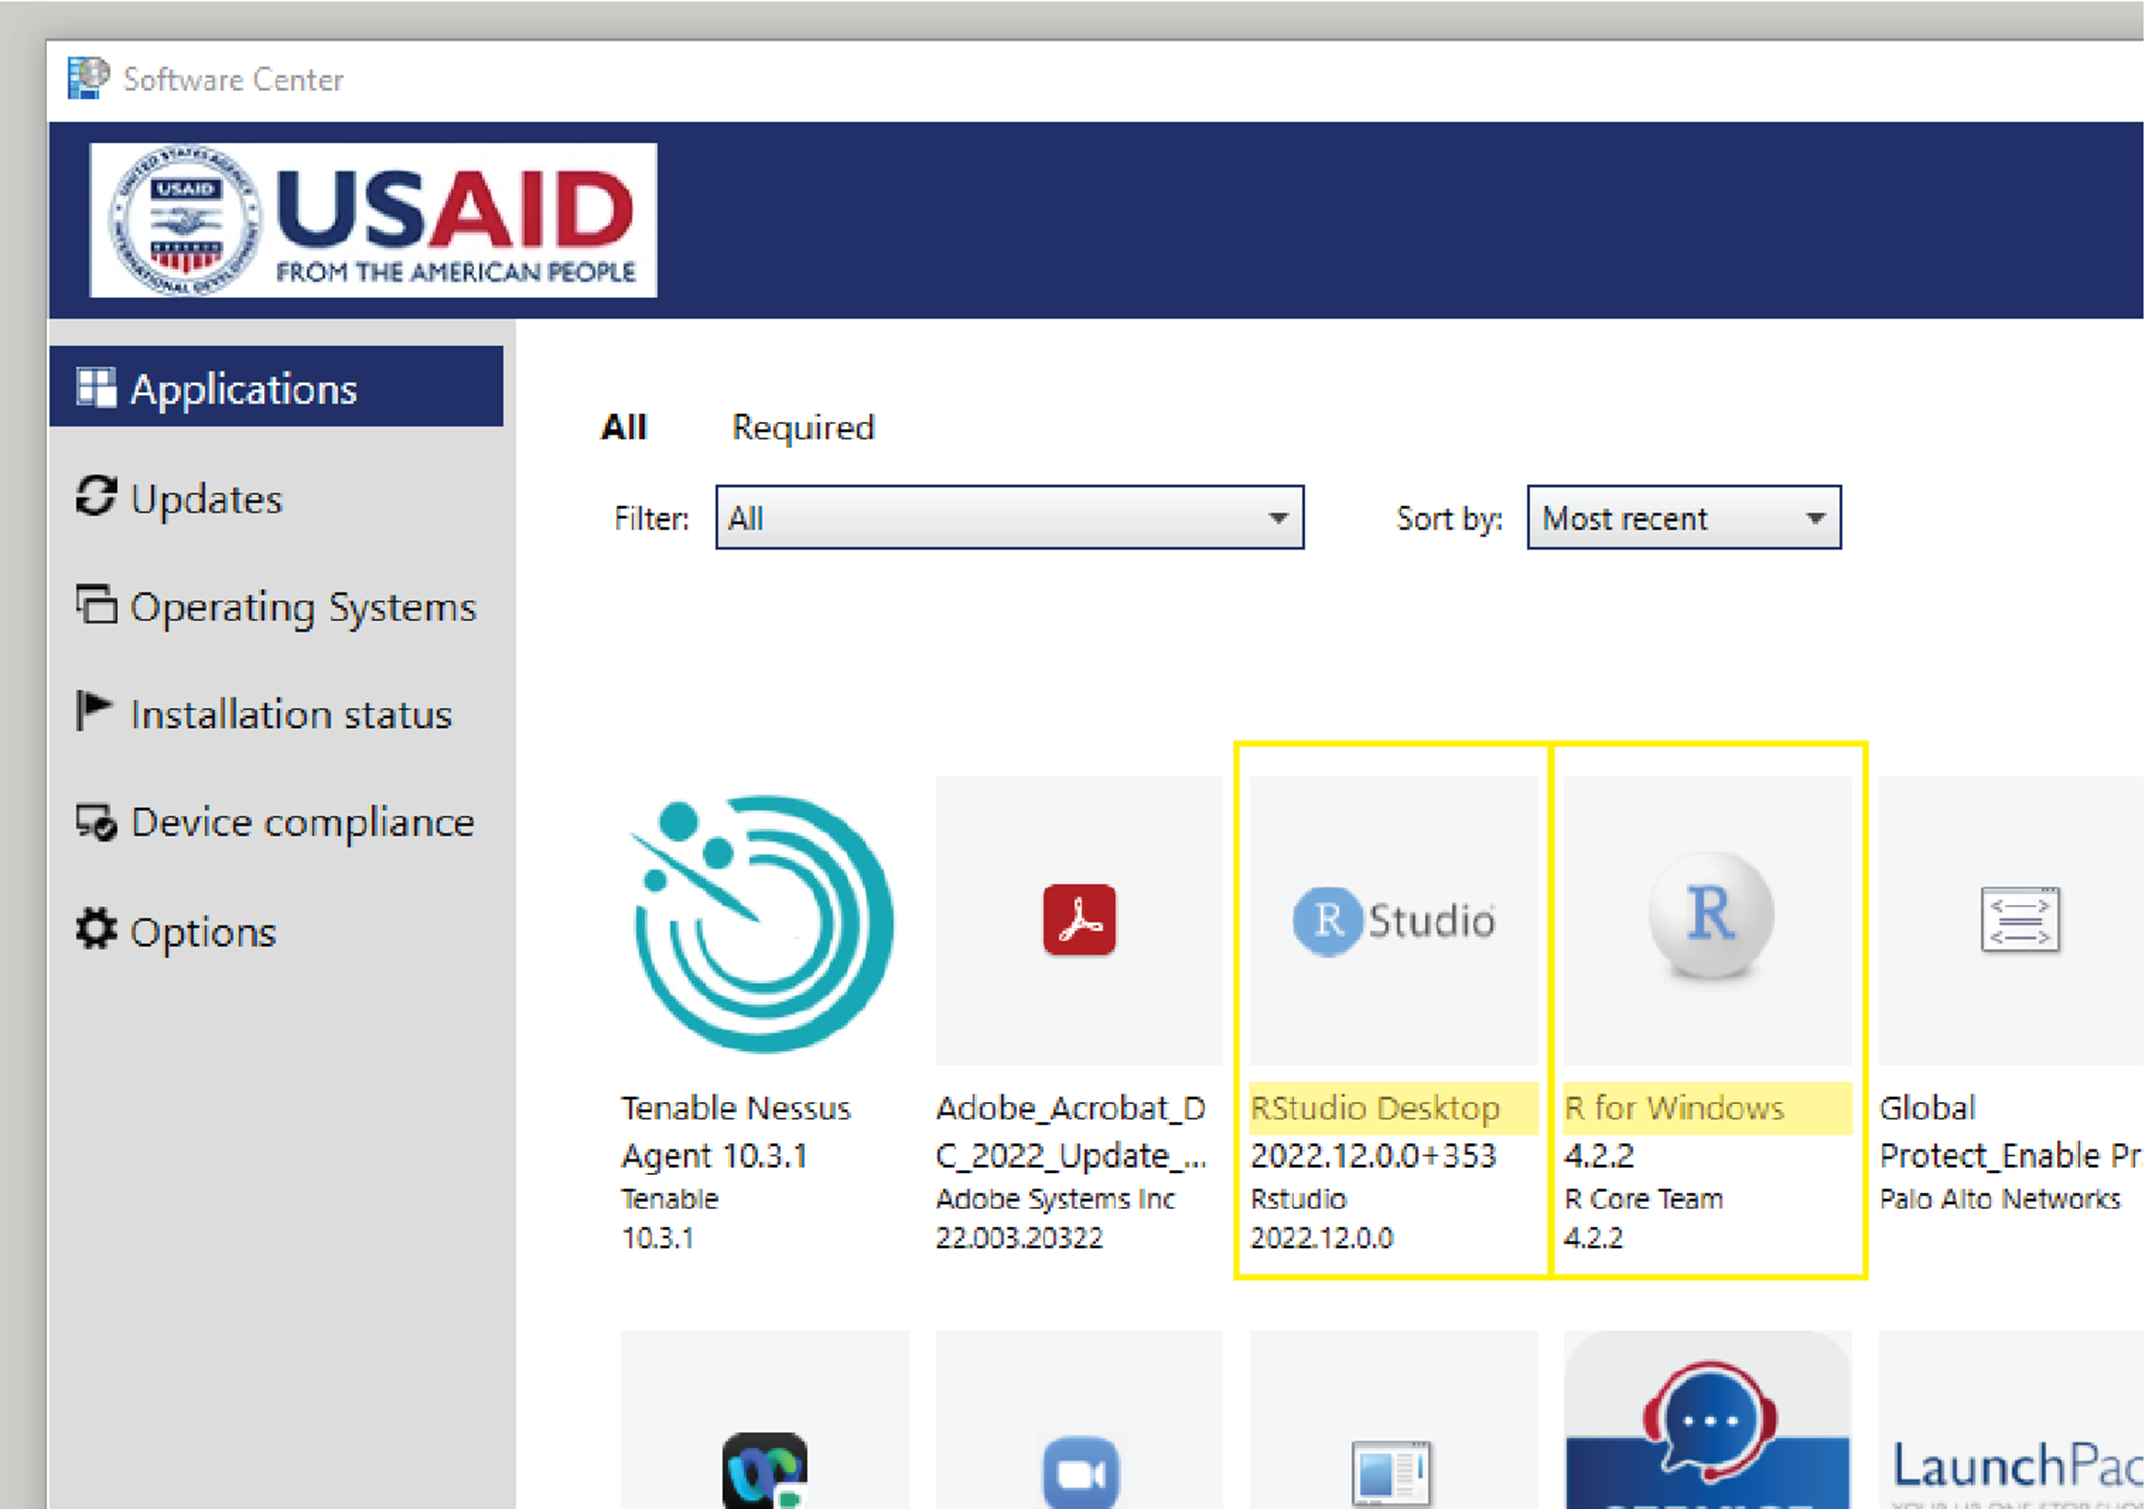
\includegraphics{./images/r_setup-software-center_r.png}

}

\end{figure}

If working on a personal machine, you can install R from
\href{https://cran.r-project.org/}{CRAN}. Select ``Download R for
Windows'' and then ``base'' and follow the instructions for installing
that pop up when you launch the .exe file from your downloads. RStudio
Desktop can be installed
\href{https://posit.co/download/rstudio-desktop/}{Posit's website} by
selecting ``Download RStudio Desktop for Windows'' and then following
the setup instructions.

\hypertarget{installing-rtools}{%
\section{Installing Rtools}\label{installing-rtools}}

If you are working on a GFE, you will need to submit a ticket to
\href{CIO-HELPDESK@usaid.gov}{M/CIO Help Desk} to install Rtools on your
machine. If you are installing from your personal machine, you will need
to \href{https://cran.r-project.org/bin/windows/Rtools/}{download} and
install the version of Rtools based on the R version you are using. You
can determine what version of R you are using by opening up a new
instance of R or RStudio and the version will be the very first thing
that appears in your console.

\hypertarget{rstudio-global-options}{%
\section{RStudio Global Options}\label{rstudio-global-options}}

It's best practice to start with a clean session each time you load up
RStudio, so you will want to adjust some default options in your IDE. To
access these, in the menu bar at the top, navigate to Tools
\textgreater{} Global Options. Here are the places you will want to make
changes to the default options before you hit ``Apply'':

\begin{itemize}
\tightlist
\item
  Uncheck ``Result most recent opened project at startup''
\item
  Uncheck ``Restore .RData into Workspace at startup''
\item
  Change dropdown to ``Never'' for ``Save workspace to .RData on exit''
\item
  Uncheck ``Always save history (even when not saving .RData)
\end{itemize}

\begin{figure}

{\centering 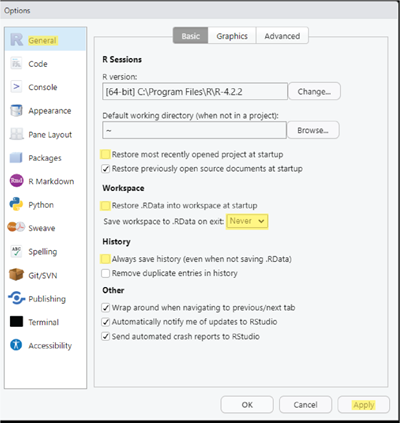
\includegraphics{./images/r_setup-global-options.png}

}

\end{figure}

\hypertarget{storing-snippets}{%
\section{Storing Snippets}\label{storing-snippets}}

Rstudio code snippets are predefined code shortcuts that can be used to
quickly insert commonly used code blocks. The use of snippets can
improve coding efficiency, reduce the time spent copying and pasting
code from other scripts, and improve the readability of your code by
providing a standardized format for your analytical scripts.

To create your own snippets in Rstudio, go to ``Tools \textgreater{}
Global Options \textgreater{} Code \textgreater{} Edit Snippets. This
will open a file where you can define your custom snippets using a
simple syntax.

\begin{figure}

{\centering 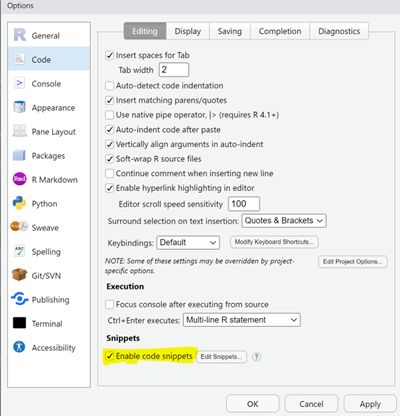
\includegraphics{./images/r_setup-snippets_global-options.png}

}

\end{figure}

Rstudio comes bundled with a set of built-in snippets that you may have
already used without even realizing it. The snippets are not limited to
just R, but to all of the different languages you can code in within the
Rstudio IDE. In the example below, this snippet sets up the formatting
of a script for you. To create a new snippet, follow the syntax in the
window and click save. Your snippet is now available for use.

\begin{figure}

{\centering 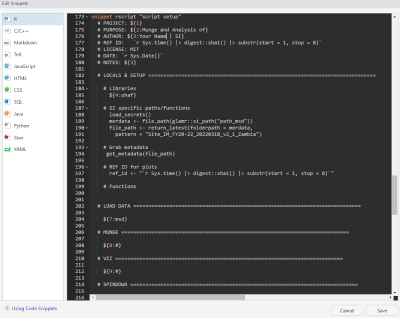
\includegraphics{./images/r_setup-snippet-window.png}

}

\end{figure}

For example, if we wanted to create snippet to insert a new object that
represents the time right now, we could use the following snippet:

\begin{verbatim}
snippet time “insert time right now”     
   Sys.time()
\end{verbatim}

Close your snippet window by hitting save, and return to the console.

When we start typing we will then see the following appear.

\begin{figure}

{\centering 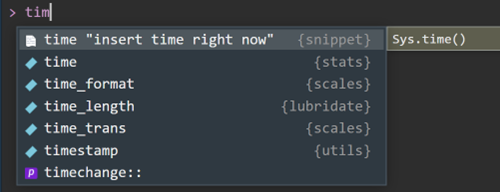
\includegraphics{./images/r_setup-snippet_insert.png}

}

\end{figure}

If we hit Tab, the \texttt{Sys.time()} function will be inserted in the
console window. When we hit enter, Rstudio will report the current time.
While this may not be that useful, you can imagine how useful this may
be if you need to insert the date or a repeated chunk of code.

\hypertarget{types-of-snippets}{%
\section{Types of snippets}\label{types-of-snippets}}

There are broadly four different types of snippets available for use or
creation.

\begin{enumerate}
\def\labelenumi{\arabic{enumi})}
\tightlist
\item
  Predefined snippets: RStudio comes with several built-in snippets for
  common programming tasks. These snippets cover a wide range of R code
  structures and functions, such as for loops, if statements, function
  definitions, and more.
\item
  Triggering snippets: Snippets are triggered by typing a specific
  keyword followed by pressing the ``Tab'' key. For example, if you type
  ``for'' and then press ``Tab,'' RStudio will automatically expand the
  snippet into a basic for loop structure.
\item
  Tab stops: Snippets may contain tab stops (usually denoted by the
  \$\{1\}), indicated by numbers or placeholders. These allow you to
  quickly navigate through the different sections of the snippet by
  pressing the ``Tab'' key. For example, if you have a placeholder for a
  variable name, pressing ``Tab'' will move the cursor to that position,
  allowing you to enter the desired variable name.
\item
  Dynamic snippets: Snippets can be dynamic and include placeholders
  that are automatically filled with values based on the context.For
  example, the ``\# DATE: r Sys.Date()'' code chunk will insert today's
  date into your script.
\end{enumerate}

By using RStudio snippets, you can streamline your coding workflow,
reduce repetitive typing, and improve overall productivity when working
with R code. We highly encourage you to take advantage of snippets and
share your discoveries with the team.

\href{https://gist.github.com/tessam30/fc775a2f917ea5d62de0f6724c4aeada}{Link
to SI Snippets}

\hypertarget{additional-resources}{%
\section{Additional Resources}\label{additional-resources}}

\begin{itemize}
\tightlist
\item
  \href{http://jtleek.com/modules/01_DataScientistToolbox/02_10_rtools/\#1}{Installing
  Rtools - Jeffrey Leek}
\item
  \href{https://usaid-oha-si.github.io/corps/rbbs/2022/01/28/rbbs-0-setup.html}{RBBS
  - 0 Software and Account Setup: Setting up Rtools - Aaron Chafetz}
\end{itemize}

\hypertarget{installing-source-sans-pro-typeface}{%
\chapter{Installing Source Sans Pro
Typeface}\label{installing-source-sans-pro-typeface}}

To create standard visualizations across our SI team, we rely on one of
USAID's alternate fonts,
\href{https://fonts.google.com/specimen/Source+Sans+Pro}{Sans Source
Pro}. This typeface is not only not native to R, nor is it a standard to
Windows, but is an open source typeface available from Google Fonts.

\begin{figure}

{\centering 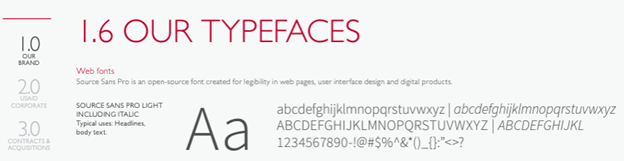
\includegraphics{./images/typeface_setup-usaid-style_font.png}

}

\end{figure}

To install the font on your GFE, you can find it in Software Center
(Start \textgreater{} Microsoft Endpoint manager \textgreater{} Software
Center). Once there, you can select the Application called ``Source Sans
Pro'' and click ``Install''.

\begin{figure}

{\centering 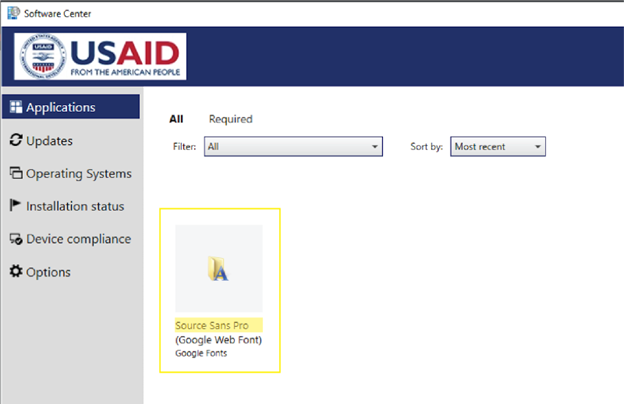
\includegraphics{./images/typeface_setup-software-center_font.png}

}

\end{figure}

To install it on your computer, navigate to the typeface on
\href{https://fonts.google.com/specimen/Source+Sans+Pro}{Google Fonts}
and click the ``Download family''. After the folder finishes
downloading, unzip it.

\hypertarget{accessing-fonts-in-r}{%
\section{Accessing Fonts in R}\label{accessing-fonts-in-r}}

To use non-native fonts in R, you must run a program called
\texttt{extrafonts}. You will need to run the following code below to
install all the fonts on your computer (if desired) and the one you just
downloaded/added. You will only need to import fonts only once on your
machine. However, to use these fonts with any plotting in R, you will
need to load the \texttt{extrafont} as with any other package.

\begin{verbatim}
#load library (install if these are not already installed)
library(extrafont)  #install.packages("extrafont")
library(remotes)  #install.packages("remotes")

#downgrade a package dependency for extrafont
#https://stackoverflow.com/questions/61204259/how-can-i-resolve-the-no-font-name-issue-when-importing-fonts-into-r-using-ext/68642855#68642855
install_version("Rttf2pt1", version = "1.3.8")

#import all Windows fonts
  font_import()
  
#restart your R session - CTRL + SHIFT + F10

#check that your fonts are now accessible in R
library(extrafont)
fonts()
\end{verbatim}

\begin{figure}

{\centering 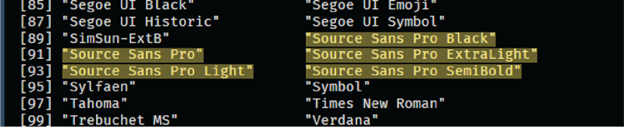
\includegraphics{./images/typeface_setup-typeface_installed.png}

}

\end{figure}

\hypertarget{additional-resources-1}{%
\section{Additional Resources}\label{additional-resources-1}}

\begin{itemize}
\tightlist
\item
  \href{https://www.usaid.gov/branding/gsm}{USAID Graphic Standards
  Manual}
\item
  \href{https://fonts.google.com/specimen/Source+Sans+Pro}{Google Fonts:
  Sans Source Pro}
\item
  \href{https://stackoverflow.com/questions/61204259/how-can-i-resolve-the-no-font-name-issue-when-importing-fonts-into-r-using-ext/68642855\#68642855}{Stack
  Overflow: Resolve the ``No Font Name Issue''}
\item
  \href{https://usaid-oha-si.github.io/glitr/}{glitr package}
\end{itemize}

\hypertarget{installing-git-git-client}{%
\chapter{Installing git \& git client}\label{installing-git-git-client}}

GitHub serves as a platform for hosting code, facilitating version
control, and enabling collaborative work. It empowers you and your team
to collaborate on projects seamlessly, regardless of your physical
location. To begin using Git and GitHub, a series of essential steps
must be followed to set up and initialize the Git environment:

This can be done at the GitHub website where you can sign up for an
account for free. While you can use your USAID email, you might want to
consider using a personal email to maintain access to your work should
you leave USAID. Once that is created, you will need to be added to the
``USAID-OHA-SI'' organization and appropriate teams, which will be
further outlined in \emph{{[}insert chapter name{]}}\_\_.

\hypertarget{install-or-upgrade-r-and-rstudio}{%
\section{Install or upgrade R and
RStudio}\label{install-or-upgrade-r-and-rstudio}}

Assuming that you've installed R and R Studio as outlined \_\_\_, it is
best to make sure that your installation is upgraded to the most current
version. This ensures that you have all of the latest functionality and
resources.

To make sure your R installation is current, you can check in the
``Console'':

\begin{Shaded}
\begin{Highlighting}[]
\CommentTok{\# Check what version of R \& Rstudio you are using. Try to use the most recent versions.}
\NormalTok{R.version.string}
\end{Highlighting}
\end{Shaded}

\begin{verbatim}
[1] "R version 4.2.2 (2022-10-31 ucrt)"
\end{verbatim}

\begin{Shaded}
\begin{Highlighting}[]
\CommentTok{\#   Check version of R{-}studio}
\CommentTok{\#Rstudio.Version()}
\CommentTok{\#rstudioapi::getVersion()}
\end{Highlighting}
\end{Shaded}

\hypertarget{setting-up-a-project}{%
\chapter{Setting up a project}\label{setting-up-a-project}}

An R project is a directory that contains all the contents, scripts, and
resources that are related to a specific project. R projects enable us
to group our work into self-contained folders, which is particularly
useful if we have context-specific analyses that we wish to keep
distinct.

The most beneficial aspect of creating an R Project is that the working
directory is the project's roots folder - this allows us to keep track
of all the files that are pertinent to a specific project and easily
read files from the working directory. It also allows us the ability to
preserve our workspace between sessions.

When a project is created, RStudio will create a new R session for the
project. It will allow create the following files:

\begin{itemize}
\tightlist
\item
  An \textbf{.Rproj} file in the project's main directory, which
  contains the same working directory, R session, and command history.
  Previous edited documents and files are restored in editor tabs, as
  well.
\item
  An \textbf{.Rhistory} file in the project's main directory, which
  contains the command history from your session that is loaded into the
  R Project
\item
  An \textbf{.Rdata} file in the project's main directory, which
  contains the data and changes from your sessions to be loaded in the R
  Project
\end{itemize}

\begin{enumerate}
\def\labelenumi{\arabic{enumi}.}
\item
  Open RStudio and go to the File menu and select \texttt{New\ Project}.
\item
  In the \texttt{New\ Project} window, choose \texttt{New\ Directory}.
  Then, choose \texttt{New\ Project}. Name your new directory and then
  ``Create the project as subdirectory of'' and select a folder on your
  computer (preferably your folder where you will store all of your R
  Projects). Click on Create Project.
\item
  After your project is completed, if the project does not automatically
  open in RStudio, then go to the File menu, select Open Project, and
  choose the file with the extension \texttt{.Rproj}.
\item
  When RStudio opens, you will see three panels in the window.~ Verify
  your working directory now that we have our Project set up using
  \texttt{getwd()}.
\end{enumerate}

\textbf{Note}: If your RStudio is already opened from an existing
project, you may want to check the \texttt{Open\ in\ a\ new\ session}
checkbox to open the project in a new session.

\hypertarget{installing-our-base-set-of-packages}{%
\chapter{Installing our base set of
packages}\label{installing-our-base-set-of-packages}}

Whereas programs like Stata, SPSS, etc come with a full suite of built
in functions, R is an open source tool with contributions from users all
over the globe. There are some built in functions that come preloaded
with R, but for the most part, you will rely on package from other
contributors. There are tons and tons of packages available on CRAN and
even more hosted elsewhere, like on GitHub. It can be a bit intimidating
to figure out what packages to install from the start, so we will
suggest a handful that we use all the time.

\begin{itemize}
\tightlist
\item
  \textbf{\texttt{dplyr}}: A fast, consistent tool for working with data
  frame like objects, both in memory and out of memory
\item
  \textbf{\texttt{tidyr}} : Tools to help to create tidy data, where
  each column is a variable, each row is an observation, and each cell
  contains a single value. `tidyr' contains tools for changing the shape
  (pivoting) and hierarchy (nesting and `unnesting') of a dataset,
  turning deeply nested lists into rectangular data frames
  (`rectangling'), and extracting values out of string columns. It also
  includes tools for working with missing values (both implicit and
  explicit).
\item
  \textbf{\texttt{ggplot2}}: A system for `declaratively' creating
  graphics, based on The Grammar of Graphics''. You provide the data,
  tell `ggplot2' how to map variables to aesthetics, what graphical
  primitives to use, and it takes care of the details.
\item
  \textbf{\texttt{readr}}: The goal of `readr' is to provide a fast and
  friendly way to read rectangular data (like `csv', `tsv', and `fwf').
  It is designed to flexibly parse many types of data found in the wild,
  while still cleanly failing when data unexpectedly changes
\item
  \textbf{\texttt{readxl}}: Import excel files into R. Supports `.xls'
  via the embedded \href{https://github.com/libxls/libxls}{`libxls' C
  library} and `.xlsx' via the embedded
  \href{https://rapidxml.sourceforge.net/}{`RapidXML' C++ library}.
\item
  \textbf{\texttt{forcats}}: Helpers for reordering factor levels
  (including moving specified levels to front, ordering by first
  appearance, reversing, and randomly shuffling), and tools for
  modifying factor levels (including collapsing rare levels into other,
  `anonymising', and manually `re-coding').
\item
  \textbf{\texttt{stringr}}: A consistent, simple and easy to use set of
  wrappers around the fantastic `stringi' package. All function and
  argument names (and positions) are consistent, all functions deal with
  NA's and zero length vectors in the same way, and the output from one
  function is easy to feed into the input of another.
\item
  \textbf{\texttt{lubridate}}: Functions to work with date-times and
  time-spans: fast and user friendly parsing of date-time data,
  extraction and updating of components of a date-time (years, months,
  days, hours, minutes, and seconds), algebraic manipulation on
  date-time and time-span objects.
\item
  \textbf{\texttt{reprex}}: Convenience wrapper that uses the
  `rmarkdown' package to render small snippets of code to target formats
  that include both code and output.
\item
  \textbf{\texttt{tidyverse}}: The `tidyverse' is a set of packages that
  work in harmony because they share common data representations and
  `API' design. This package is designed to make it easy to install and
  load multiple `tidyverse' packages in a single step.
\item
  \textbf{\texttt{googledrive}}: Manage Google Drive files from R.
\item
  \textbf{\texttt{glue}}: An implementation of interpreted string
  literals, inspired by
  \href{https://www.python.org/dev/peps/pep-0498/}{Python's Literal
  String Interpolation} and
  \href{https://www.python.org/dev/peps/pep-0257/}{Docstrings} and
  \href{https://docs.julialang.org/en/v1.3/manual/strings/\#Triple-Quoted-String-Literals-1}{Julia's
  Triple-Quoted String Literals}
\end{itemize}

\hypertarget{other-packages}{%
\section{\texorpdfstring{\emph{Other
Packages}}{Other Packages}}\label{other-packages}}

\begin{itemize}
\tightlist
\item
  \textbf{`remotes'}: Download and install R packages stored in
  `GitHub', `GitLab', `Bitbucket', `Bioconductor', or plain `subversion'
  or `git' repositories.
\item
  \textbf{\texttt{scales}}: Graphical scales map data to aesthetics, and
  provide methods for automatically determining breaks and labels for
  axes and legends.
\item
  \textbf{\texttt{extrafont}}: Tools to using fonts other than the
  standard PostScript fonts. This package makes it easy to use system
  TrueType fonts and with PDF or PostScript output files, and with
  bitmap output files in Windows.
\item
  \textbf{\texttt{patchwork}}: The `ggplot2' package provides a strong
  API for sequentially building up a plot, but does not concern itself
  with composition of multiple plots. `patchwork' is a package that
  expands the API to allow for arbitrarily complex composition of plots
  by, among others, providing mathematical operators for combining
  multiple plots.
\item
  \textbf{\texttt{datapasta}}: RStudio addins and R functions that make
  copy-pasting vectors and tables to text painless.
\item
  \textbf{\texttt{quickview}}: RStudio addin to quickly inspect data in
  a View tab or open them with default CSV/text editor software.
\end{itemize}

\hypertarget{ohasi-packages}{%
\section{\texorpdfstring{\emph{OHA/SI
Packages}}{OHA/SI Packages}}\label{ohasi-packages}}

\begin{itemize}
\tightlist
\item
  \textbf{\texttt{glitr}}: Helps create and export ggplot2 charts in the
  style used by the GH OHA SI team. Includes multiple styles and themes
  to tweak plots to user needs. Sample testing data also available.
\item
  \textbf{\texttt{glamr}}: Provides a series of base functions useful to
  the GH OHA SI team. This includes project setup, pulling from DATIM,
  and key functions for working with the MSD.
\item
  \textbf{\texttt{gisr}}: R Spatial functions for HIV/AIDS related
  Geospatial Analytics
\item
  \textbf{\texttt{gagglr}}: Since package are developed with a regular
  update cycle, users can often be using outdated packages that resolve
  bug or add new features. This checks to ensure you are using the
  lastest version of the OHA core package and allows you to load them
  all at the start of a session. This package borrows heavily from the
  tidyverse package.
\item
  \textbf{\texttt{tameDP}}: Import PSNUxIM targets and PLHIV data from
  COP Data Pack. The purpose is to make the data tidy and more usable
  than their current structure in the Excel data packs.
\end{itemize}

Whenever you are installing packages, you should start from a clean
instance of R and not load any packages until you are finished
installing what you want. Most packages are found on CRAN and require a
simpler means of installation; others found on GitHub and elsewhere
require a different function to install, specifying the source and
repository.

\begin{verbatim}
#tidyverse packages (all)
install.packages("tidyverse")

#other packages
install.packages("remotes")
install.packages("scales")
install.packages("extrafont")
install.packages("patchwork")
remotes::install_github("MilesMcBain/datapasta")
remotes::install_github("fkeck/quickview")

#USAID-OHA-SI packages
remotes::install_github("USAID-OHA-SI/glitr")
remotes::install_github("USAID-OHA-SI/glamr")
remotes::install_github("USAID-OHA-SI/gisr")
remotes::install_github("USAID-OHA-SI/gagglr")
remotes::install_github("USAID-OHA-SI/tameDP")
\end{verbatim}

\hypertarget{additional-resources-2}{%
\section{Additional Resources}\label{additional-resources-2}}

\begin{itemize}
\tightlist
\item
  \href{https://www.tidyverse.org/}{The Tidyverse Packages}
\item
  \href{https://posit.co/resources/cheatsheets/}{Posit Cheatsheets}
\item
  \href{https://usaid-oha-si.github.io/tools/}{OHA Packages}
\end{itemize}

\hypertarget{credential-management}{%
\chapter{Credential management}\label{credential-management}}

While the large majority of our analytic work is using local flat files,
SI analysts have access to a number of different platforms including
PEPFAR DATIM, PEPFAR Panorama, UNAIDS AIDSInfo, USAID Google Drive, and
the USAID's Data Development Commons (DDC) all with their own set of
credentials. \textbf{Passwords, user names, and access keys should never
be stored in scripts}, regardless of whether the script is saved locally
or made available on GitHub. To help ensure this safety measure while
also maximizing reproducibility across our team, we rely on a set of
functions within our inhouse packages,
\href{https://usaid-oha-si.github.io/glamr/}{\texttt{glamr}}. Using
\texttt{glamr} systematize USAID analysts code, calling objects the same
way and in the same locations across machines.

Let's go through an example of how this might be used, starting by
loading the \texttt{glamr} package.

\begin{Shaded}
\begin{Highlighting}[]
\FunctionTok{library}\NormalTok{(glamr)}
\end{Highlighting}
\end{Shaded}

Before using credentials you'll need to store them on your local OS. The
\texttt{glamr} package utilizes the \texttt{keyring} package to store
and access the usernames and passwords, storing this information in
Windows' Credential Store.

Let's start by storing our USAID email address, which we will use to
access Google Drive. You'll only be storing your email, not password, as
this is authenticated via standard OAuth2 browser flow. The
\texttt{set\_email()} function also helps you to store your email in
your \texttt{.Rprofile}, allowing \texttt{googledrive::drive\_auth()}
and \texttt{googlesheets4::gs4\_auth()} to run without you having to
enter your email.

\begin{Shaded}
\begin{Highlighting}[]
\FunctionTok{set\_email}\NormalTok{(}\StringTok{"spower@usaid.gov"}\NormalTok{)}
\end{Highlighting}
\end{Shaded}

Next up we'll store our DATIM credentials. For this, you'll need to
enter your DATIM username. When you run the code, you will get a
prompt/pop-up window in RStudio to enter your DATIM password.

\begin{Shaded}
\begin{Highlighting}[]
\FunctionTok{set\_datim}\NormalTok{(}\StringTok{"spower"}\NormalTok{)}
\end{Highlighting}
\end{Shaded}

You can also store your PEPFAR Panorama credential, allowing you to
access and download the PEPFAR Structured Datasets. For this, you'll
need to enter your Panorma username. When you run the code, you will get
a prompt/pop-up window in RStudio to enter your Panoma password.

\begin{Shaded}
\begin{Highlighting}[]
\FunctionTok{set\_pano}\NormalTok{(}\StringTok{"spower@usaid.gov"}\NormalTok{)}
\end{Highlighting}
\end{Shaded}

Lastly, if you have access to an Amazon Web Services (s3) account, you
can also store your s3 access and secret keys, which will prompt for the
key and secret.

\begin{Shaded}
\begin{Highlighting}[]
\FunctionTok{set\_account}\NormalTok{(}\AttributeTok{name =}\NormalTok{ “s3”)}
\end{Highlighting}
\end{Shaded}

These functions have now passed your credentials in your operating
system's credential manager - Credential Store on Windows and Keychain
on MacOS. We can use \texttt{keyring} to see all the ``services'', or
accounts, stored on your machine.

\begin{Shaded}
\begin{Highlighting}[]
\NormalTok{keyring}\SpecialCharTok{::}\FunctionTok{key\_list}\NormalTok{()}
\end{Highlighting}
\end{Shaded}

\hypertarget{old-way-of-doing-things}{%
\section{Old way of doing things}\label{old-way-of-doing-things}}

Without using the \texttt{glamr} package, analysts would have had to
write out their username and authenticate. Prior to saving and pushing
the code to GitHub, the analyst would have to remove their email.
Another analyst would have to review the code and find where to put
their email in manually if running themselves.

\begin{Shaded}
\begin{Highlighting}[]
\FunctionTok{library}\NormalTok{(googlesheets4)}

\CommentTok{\#email}
\NormalTok{  email }\OtherTok{\textless{}{-}} \StringTok{"spower@usaid.gov"} 

\CommentTok{\#authenticate}
  \FunctionTok{gs4\_auth}\NormalTok{(email)}

\CommentTok{\#specific Google Sheet Unique ID (found at the end of the URL)}
\NormalTok{  sheet\_id }\OtherTok{\textless{}{-}} \StringTok{\textquotesingle{}5mD3ndk08Sdd3dn1dm29smD\textquotesingle{}}
  
\CommentTok{\#read directly into R (similar to read\_csv or read\_xlsx)}
\NormalTok{  df }\OtherTok{\textless{}{-}} \FunctionTok{read\_sheet}\NormalTok{(}\FunctionTok{as\_sheets\_id}\NormalTok{(sheet\_id), }\StringTok{"Sheet1"}\NormalTok{)  }
\end{Highlighting}
\end{Shaded}

We faced a similar issue with DATIM credentials, where we had to either
write out our username and remove prior to pushing to GitHub or some
analysts stored this information in scripts in different locations on
their different machines, using different object name, eg \texttt{user},
\texttt{myuser}, \texttt{datim\_acct}, \texttt{datim\_login}, etc.

\begin{Shaded}
\begin{Highlighting}[]
\CommentTok{\#DATIM user}
\NormalTok{  user }\OtherTok{\textless{}{-}} \StringTok{"spower"}

\CommentTok{\#pull DATIM table of OU/country UIDs and sub{-}national unit levels}
\NormalTok{  ou\_table }\OtherTok{\textless{}{-}} \FunctionTok{datim\_outable}\NormalTok{(user, }\FunctionTok{mypwd}\NormalTok{(user))}
\end{Highlighting}
\end{Shaded}

\hypertarget{accessing-stored-credentials}{%
\section{Accessing stored
credentials}\label{accessing-stored-credentials}}

The old way of doing things was inefficient and posed a risk of posting
credentials accidentally. The previous method required storing the
username in your code and then using it to pull from an encrypted local
file that stored the password associated with the username using
\texttt{glamr::mypwd()}. Each analyst would have to change the username
if they ran the code. The analyst, now, will perform the same task, but
won't have to write out their username in the code since it's loaded
into the session with \texttt{load\_secrets()} and always
assigned/called the same thing.

Now that they're stored after using \texttt{set\_email()} and
\texttt{set\_datim()}, we can load up our credentials at the beginning
of our code and be available for your current R session. In addition to
storing your email, \texttt{load\_secrets()} will authenticate with
Google Drive if you have the \texttt{googledrive} and/or
\texttt{googlesheets4} packages.

\begin{Shaded}
\begin{Highlighting}[]
\FunctionTok{load\_secrets}\NormalTok{()}
\end{Highlighting}
\end{Shaded}

Your account information is stored for the session in \texttt{Options}
and can be accessed directly via \texttt{getOptions("email")} or
\texttt{getOptions("datim")}. We also have two wrapper functions to pull
your DATIM information since you may need to include that in an API
request - \texttt{datim\_user()} and \texttt{datim\_pwd()}

How does this help? Instead of having to manually enter your USAID
email, it can be loaded automatically and already authenticated for
Google API by running \texttt{load\_secrets()}. The user can also
specify which authentication they want to provide in a session, rather
than loading all of them. For example, you could just specify to
authenticate for use with Google Drive and Sheets -
\texttt{load\_secrets("email")}.

\begin{Shaded}
\begin{Highlighting}[]
\FunctionTok{library}\NormalTok{(googlesheets4)}
\FunctionTok{library}\NormalTok{(glamr)}

\CommentTok{\#setup session}
  \FunctionTok{load\_secrets}\NormalTok{()}

\CommentTok{\#specific Google Sheet Unique ID (found at the end of the URL)}
\NormalTok{  sheet\_id }\OtherTok{\textless{}{-}} \StringTok{\textquotesingle{}5mD3ndk08Sdd3dn1dm29smD\textquotesingle{}}

\CommentTok{\#read directly into R (similar to read\_csv or read\_xlsx)}
\NormalTok{  df }\OtherTok{\textless{}{-}} \FunctionTok{read\_sheet}\NormalTok{(}\FunctionTok{as\_sheets\_id}\NormalTok{(sheet\_id), }\StringTok{"Sheet1"}\NormalTok{)}
  
\CommentTok{\#pull DATIM table of OU/country UIDs and sub{-}national unit levels}
\NormalTok{  ou\_table }\OtherTok{\textless{}{-}} \FunctionTok{datim\_outable}\NormalTok{(}\FunctionTok{datim\_user}\NormalTok{(), }\FunctionTok{datim\_pwd}\NormalTok{())}
\end{Highlighting}
\end{Shaded}

\part{Working with data}

\hypertarget{storing-and-accessing-pepfar-data}{%
\chapter{Storing and accessing PEPFAR
data}\label{storing-and-accessing-pepfar-data}}

When working on any given project, the general advice is typically to
store your data in that specific project 's repository. This advice is a
good best practice, but does not translate well in the PEPFAR space for
two main reasons: file size and sensitivity. Instead, we recommend
storing PEPFAR structured datasets in a centralized location on your
machine outside of the project,
e.g.~\texttt{C:\textbackslash{}Users\textbackslash{}spower\textbackslash{}Documents\textbackslash{}Data}.

Our work primarily revolves around using PEPFAR structured datasets,
which are large, cumbersome SQLview output files, e.g.~OUxIM, PSNU,
PSNUxIM, NAT\_SUBNAT, and FSD. Given this fact, it makes more sense for
us to store these dataset in a central location on our machines rather
than duplicating these files in each project. These PEPFAR structured
datasets are easily accessible for anyone working in PEPFAR, either from
\href{https://pepfar-panorama.org/}{PEPFAR Panorama} or through the
\href{https://www.datim.org/}{DATIM Genie}.

The second reason for storing these datasets outside of the project is
to avoid any risk of posting these non-public data to a public space
when using version control. While these structured dataset are
aggregated and not individual patient level data, they are not published
by PEPFAR to the public and may contain sensitivities when it comes to
key populations or when using data at the facility level.

For small (and non-PEPFAR structured) datasets, we recommend storing
these data within the project either in the \texttt{Data} and
\texttt{Data\_public} folder. Another alternative is storing the data on
Google Drive in a shared folder and pulling the data down utilizing the
Google API via the \texttt{googledrive} or \texttt{googlesheets4}
packages.

\hypertarget{accessing-pepfar-data}{%
\section{Accessing PEPFAR Data}\label{accessing-pepfar-data}}

PEPFAR maintains a number of different structured datasets across MER,
EA, Budget, and SIMS. Data are entered into DATIM, the system of record,
by partners and goes through an approval process that takes about six
weeks after the quarter ends. In-process data can be accessed through
DATIM and the \href{https://www.datim.org/}{DATIM Genie}, which will
export data in the typical structured manner. Otherwise, datasets are
made available on \href{https://pepfar-panorama.org/}{PEPFAR Panorama}
for download. PEPFAR data can also be pulled directly from DATIM
utilizing an API (see the
\href{https://docs.dhis2.org/en/develop/using-the-api/dhis-core-version-240/introduction.html}{DHIS2
API documentation} or our
\href{https://usaid-oha-si.github.io/grabr/}{\texttt{grabr} package}

As mentioned in the last section, we recommend storing these datasets in
a central location on your computer. This creates a problem from a
collaboration standpoint, as we can't just point to the ``Data'' folders
in our project using a relative path; we have to provide a file path
that only works on one user's machine and not another. To solve this
dilemma, we use a function in the
\href{https://usaid-oha-si.github.io/glamr}{\texttt{glamr} package}
called \texttt{si\_paths()} which access the paths we have stored
locally to where our PEPFAR structured datasets reside. This way, when
you pick up a coworker's code, you don't have to change any of the file
paths, it just works.

Those local paths need to be set once and stored in your
\texttt{.Rprofile}. To do so, you will run \texttt{glamr::set\_paths()}
to store all the relevant paths (you can ignore any that aren't relevant
to you). The below example would be the code I would run in the console
indicating where my folders are for the MSD, DATIM files and Downloads.

\begin{Shaded}
\begin{Highlighting}[]
\FunctionTok{library}\NormalTok{(glamr)}
\FunctionTok{set\_paths}\NormalTok{(}\AttributeTok{folderpath\_msd =} \StringTok{"\textasciitilde{}/Documents/Data"}\NormalTok{,}
  \AttributeTok{folderpath\_datim =}  \StringTok{"\textasciitilde{}/Documents/DATIM"}\NormalTok{,}
  \AttributeTok{folderpath\_downloads =}  \StringTok{"\textasciitilde{}/Downloads"}\NormalTok{)}
\end{Highlighting}
\end{Shaded}

\hypertarget{additional-resources-3}{%
\section{Additional Resources}\label{additional-resources-3}}

\begin{itemize}
\tightlist
\item
  \href{https://usaid-oha-si.github.io/glamr/articles/project-workflow.html}{Project
  Workflow Vignette}
\item
  \href{https://usaid-oha-si.github.io/glamr/}{glamr package}
\item
  \href{https://usaid-oha-si.github.io/grabr/}{grabr package}
\item
  \href{https://docs.dhis2.org/en/develop/using-the-api/dhis-core-version-240/introduction.html}{DHIS2
  API Documentation}
\end{itemize}

\hypertarget{best-practices-on-writing-a-script}{%
\chapter{Best practices on writing a
script}\label{best-practices-on-writing-a-script}}

One of the big upsides of scripting is you have instance documentation
of what was one. If we can follow similar practices of commenting and
organizing our work, we will make it easier for others and our future
selves to more easily understand what is going on in your script.

R Scripts read just like documents do. We have lines of code that R
reads top-down and executes, with specific steps built off of what was
done previously.

We can organize our scripts with a similar flow to organizing a
document, to clean up the script visually and help you and others better
understand what each part of the script is used for. We can utilize
comments to add headers into our script for organization.

While there is no one right way to organize a script, here is an example
of how we tend to set up our scripts within OHA/SI. Check out the
{[}Storing Snippets Section{]} to see how you can easily add this to
beginning of each of your scripts.

\begin{itemize}
\tightlist
\item
  \textbf{Introduction}: name of author, purpose of script, date,
  reference id, notes
\item
  \textbf{Load Dependencies and Libraries}
\item
  \textbf{Define global options or functions}: set up global variables
  as well (variables you want to call on throughout the script)
\item
  \textbf{Import Data}
\item
  \textbf{Data Cleaning}
\item
  \textbf{Analysis/Visualization}
\item
  \textbf{Export}
\end{itemize}

\begin{Shaded}
\begin{Highlighting}[]
\CommentTok{\# AUTHOR:   S. Powers | USAID}
\CommentTok{\# PURPOSE:  Set up training script}
\CommentTok{\# REF ID:   c2e621bd }
\CommentTok{\# LICENSE:  MIT}
\CommentTok{\# DATE:     2022{-}09{-}14}
\CommentTok{\# UPDATED: }

\CommentTok{\# DEPENDENCIES {-}{-}{-}{-}{-}{-}{-}{-}{-}{-}{-}{-}{-}{-}{-}{-}{-}{-}{-}{-}{-}{-}{-}{-}{-}{-}{-}{-}{-}{-}{-}{-}{-}{-}{-}{-}{-}{-}{-}{-}{-}{-}{-}{-}{-}{-}{-}{-}{-}{-}{-}{-}{-}{-}{-}{-}{-}{-}{-}{-}}
  
\CommentTok{\# LOAD PACKAGES {-}{-}{-}{-}{-}{-}{-}{-}{-}{-}{-}{-}{-}{-}{-}{-}{-}{-}{-}{-}{-}{-}{-}{-}{-}{-}{-}{-}{-}{-}{-}{-}{-}{-}{-}{-}{-}{-}{-}{-}{-}{-}{-}{-}{-}{-}{-}{-}{-}{-}{-}{-}{-}{-}{-}{-}{-}{-}{-}{-}}

  \FunctionTok{library}\NormalTok{(glamr)}
  \FunctionTok{library}\NormalTok{(tidyverse)}
  

\CommentTok{\# GLOBAL VARIABLES {-}{-}{-}{-}{-}{-}{-}{-}{-}{-}{-}{-}{-}{-}{-}{-}{-}{-}{-}{-}{-}{-}{-}{-}{-}{-}{-}{-}{-}{-}{-}{-}{-}{-}{-}{-}{-}{-}{-}{-}{-}{-}{-}{-}{-}{-}{-}{-}{-}{-}{-}{-}{-}{-}{-}{-}}
    
  \CommentTok{\#Grab metadata}
\NormalTok{  msd\_source }\OtherTok{\textless{}{-}} \FunctionTok{source\_info}\NormalTok{(file\_path)}
  
\NormalTok{  ref\_id }\OtherTok{\textless{}{-}} \StringTok{"c2e621bd"}

\CommentTok{\# IMPORT {-}{-}{-}{-}{-}{-}{-}{-}{-}{-}{-}{-}{-}{-}{-}{-}{-}{-}{-}{-}{-}{-}{-}{-}{-}{-}{-}{-}{-}{-}{-}{-}{-}{-}{-}{-}{-}{-}{-}{-}{-}{-}{-}{-}{-}{-}{-}{-}{-}{-}{-}{-}{-}{-}{-}{-}{-}{-}{-}{-}{-}{-}{-}{-}{-}{-}}
  
  \CommentTok{\#IMPORT MSD}
  \FunctionTok{si\_path}\NormalTok{() }\SpecialCharTok{\%\textgreater{}\%} 
    \FunctionTok{return\_latest}\NormalTok{() }\SpecialCharTok{\%\textgreater{}\%} 
    \FunctionTok{read\_msd}\NormalTok{() }\SpecialCharTok{\%\textgreater{}\%} 
    \FunctionTok{reshape\_msd}\NormalTok{(}\AttributeTok{clean =}\NormalTok{ T)}
  

\CommentTok{\# MUNGE {-}{-}{-}{-}{-}{-}{-}{-}{-}{-}{-}{-}{-}{-}{-}{-}{-}{-}{-}{-}{-}{-}{-}{-}{-}{-}{-}{-}{-}{-}{-}{-}{-}{-}{-}{-}{-}{-}{-}{-}{-}{-}{-}{-}{-}{-}{-}{-}{-}{-}{-}{-}{-}{-}{-}{-}{-}{-}{-}{-}{-}{-}{-}{-}{-}{-}{-}}
  
\CommentTok{\# VIZ {-}{-}{-}{-}{-}{-}{-}{-}{-}{-}{-}{-}{-}{-}{-}{-}{-}{-}{-}{-}{-}{-}{-}{-}{-}{-}{-}{-}{-}{-}{-}{-}{-}{-}{-}{-}{-}{-}{-}{-}{-}{-}{-}{-}{-}{-}{-}{-}{-}{-}{-}{-}{-}{-}{-}{-}{-}{-}{-}{-}{-}{-}{-}{-}{-}{-}{-}{-}{-}}
  
\CommentTok{\# SPIN DOWN {-}{-}{-}{-}{-}{-}{-}{-}{-}{-}{-}{-}{-}{-}{-}{-}{-}{-}{-}{-}{-}{-}{-}{-}{-}{-}{-}{-}{-}{-}{-}{-}{-}{-}{-}{-}{-}{-}{-}{-}{-}{-}{-}{-}{-}{-}{-}{-}{-}{-}{-}{-}{-}{-}{-}{-}{-}{-}{-}{-}{-}{-}{-}}
\end{Highlighting}
\end{Shaded}

You'll notice a \texttt{ref\_id} being stored in the code chunk above.
Our team utilizes reference ids in our R scripts to improve our ability
to track code to specific analytic products. These reference ids are
stored in captions at the bottom of any visualizations or outputs that
are produced from our script, so we can more easily reference the
corresponding code from our code repositories. They are automatically
generated when we create scripts from a snippet template, which uses the
following code to generate a unique, 8 character id:

\begin{Shaded}
\begin{Highlighting}[]
\FunctionTok{substr}\NormalTok{(digest}\SpecialCharTok{::}\FunctionTok{sha1}\NormalTok{(}\FunctionTok{Sys.time}\NormalTok{()), }\AttributeTok{start =} \DecValTok{1}\NormalTok{, }\AttributeTok{stop =} \DecValTok{8}\NormalTok{)}
\end{Highlighting}
\end{Shaded}

\begin{verbatim}
[1] "51b320c8"
\end{verbatim}

\hypertarget{commenting-your-code}{%
\section{Commenting Your Code}\label{commenting-your-code}}

Having a script without inline comments makes it much more challenging
to debug or decipher what is going on. It is important to add comments
(text that follows a \texttt{\#}) to chunks of code to provide insights
to what is going on. There are a couple of major things to keep in mind.

First is to not over-commenting, which then makes it more challenging to
both develop and maintain, but also to debug problems. Each chunk should
be able to be described succinctly; if you require lots of explanation
your code chunk likely needs be be broken into smaller segments.

Secondly, when we add comments to a script, by default we typically
explain what is going on with our code in plain English. However, it's
much more useful to explain \textbf{why}. Instead of adding an inline
comment that you are creating a moving average of \texttt{variable\ x},
it's better to explain that you are moving average \texttt{variable\ x}
to identify outliers based on this calculation.

\hypertarget{additional-resources-4}{%
\section{Additional Resources}\label{additional-resources-4}}

\href{https://style.tidyverse.org/}{Tidyverse Style Guide}
\href{https://google.github.io/styleguide/Rguide.html}{Google's R Style
Guide} \href{https://r4ds.had.co.nz/workflow-scripts.html}{R4DS
Workflows}

\part{Resources \& Help}

\hypertarget{using-our-github-organization}{%
\chapter{Using our GitHub
organization}\label{using-our-github-organization}}

In the previous section, we layed out the importance of using version
control via git. Git is extremely useful working locally on your own
project, but becoming incredibly valuable when used as a collaboration
tool; enter
\href{https://docs.github.com/en/get-started/quickstart/hello-world}{GitHub},
which ``is a code hosting platform for version control and
collaboration. It lets you and others work together on projects from
anywhere.'' While the data we work with cannot be shared, we can take
advantage of using a ``code hosting platform'' to share our coded work
across our team (and with our future selves), improving accountability
and transparency. We have our own organizational account on GitHub,
\href{https://github.com/USAID-OHA-SI}{USAID-OHA-SI}, which hosts all of
our code and packages we've developed.

Anyone can view the code on GitHub, but in order to contribute or or
participate in issues or projects, you will need to be added to the
\href{https://github.com/USAID-OHA-SI}{USAID-OHA-SI organizational
account}. You can email one of the organization's ``owners'' - Aaron
Chafetz (achafetz@usaid.gov), Tim Essam (tessam@usaid.gov), Baboyma
Kagniniwa (bkagniniwa@usaid.gov), Karishma Srikanth
(ksrikanth@usaid.gov) - with the email address associated with your
GitHub account.

\hypertarget{search-the-organizational-space}{%
\section{Search the organizational
space}\label{search-the-organizational-space}}

GitHub is a powerful tool because it allows us to collaborate and share
our code, with others and our future selves. By committing and pushing
code, you make all of your work searchable. This feature becomes a huge
asset to others trying to learn or review how previous analyses were
run. If you go to \href{github.com}{GitHub}, our
\href{https://github.com/USAID-OHA-SI}{organization page}, or
\url{github.com/search}, you can search through all our code.

For example, if you were interested in learning about how the
\texttt{across()} function is used, you could search
\texttt{org:USAID-OHA-SI\ mutate\ across} to see all the instances of
how we are applying this function from \texttt{dplyr} or you could
search for how viral load coverage is calculated,
\texttt{org:USAID-OHA-SI\ vlc}. GitHub has a great reference document
for using the
\href{https://docs.github.com/en/search-github/github-code-search/understanding-github-code-search-syntax}{powerful
search features}.

\hypertarget{how-to-navigate}{%
\section{How to navigate}\label{how-to-navigate}}

The \href{https://github.com/USAID-OHA-SI}{USAID-OHA-SI organizational
account} hosts all of our team's R scripts and packages. Currently we
have over 100 repositories on GitHub, so finding what you are looking
for can be challenging. One thing to note as well is that we tend to use
fun names for projects. So instead of calling a project space ``COP
planning'', we come up with names loosely related, badboys, as referring
to the Will Smith and Martin Lawrence movie about two cops. It's all our
bad attempt at humor but it keeps things fun and interesting. Since the
project names are very loosely related, you can look through the
Description which will better summarize the project.

Below are a few useful repos to review/reference:

\begin{itemize}
\tightlist
\item
  groundhogday: quarterly scripts that we find ourselves needing to use
  again and again
\item
  catch-22: one off analytic requests
\item
  agitprop: high level communications visuals typically produced for the
  OHA Front Office
\end{itemize}

In addition to having R projects stored as repositories, we rely on
GitHub for hosting our R packages so everyone can access them. Each of
our packages have their own websites, built through \texttt{pkgdown},
with documentation and are easily navigable from the
\href{https://usaid-oha-si.github.io/tools/}{SI blog}.

The package pages are great resources, but sometimes you want to see the
code underlying a function or want to suggest a change via a pull
request (PR). You can find search through the USAID-OHA-SI account to
find the repository and find the code you are looking for.

\hypertarget{when-should-i-create-a-new-repo}{%
\section{When should I create a new
repo?}\label{when-should-i-create-a-new-repo}}

As you can see, we have lots of repositories that are in existence.
Repositories are essentially projects, so we can think about creating
one when our work does not easily fit into another existing repository
or is going to be large and complex and needs to stand on its own. For
example, if I review targets for Tanzania from their target setting
tool, this likely should not be its own repo, but fits either within
\texttt{badboys} (SI related support for PEPFAR COPs) or
\texttt{rebooTZ} (OHA SI support for Tanzania).

\hypertarget{how-can-i-contribute}{%
\section{How can I contribute}\label{how-can-i-contribute}}

Version control and capturing all of our coding on GitHub is important
for a number reasons:

\begin{itemize}
\tightlist
\item
  Reduces barriers to collaboration
\item
  Provides a form of back up
\item
  Captures project evolution
\item
  Experiment without fear
\item
  Commit to transparency
\end{itemize}

There are a number of ways in which you can contribute to our community
and global good.

\begin{enumerate}
\def\labelenumi{\alph{enumi}.}
\item
  \textbf{Submit an issue} - If you are running into a bug with the
  code, getting unexpected results, or have a suggestion to make, you
  can submit a ticket on GitHub. For example, if I have an issue with a
  date conversion in \texttt{glamr}, I would go to the package repo,
  github.com/USAID-OHA-SI/glamr and navigate to the ``Issues'' tab at
  the top of the repo. There I could select the green ``New issue''
  button, and clearly the descibe the issue/suggestion (check out the
  Getting Help chapter on writing a reproducible example).
\item
  \textbf{Contribute code or a fix to an existing repo/package} - If you
  have written your own code, you can submit a pull request (PR) on
  github to get it added to the repo. When working on a shared project,
  it's best practice to work on your own branch and then submit a PR to
  get that branch included in the repo. Clone the repo to your RStudio
  and then create (checkout) a new branch (this can be done through the
  git IDE tab within RStudio or can be done in the terminal in RStudio,
  e.g git \texttt{checkout\ -b\ dev\_fix-that-thing}). Once you have
  made the changes and verified the code runs as intended, you can push
  your branch. At that stage, you can go to the repo on GitHub, navigate
  to the ``Pull requests'' tab and then create a new pull request from
  your dev branch to the main branch. The project or package
  owner/maintainer will review the PR for inclusion into the repo.
\item
  \textbf{Creating a new repo }: If you have a new project that does not
  exist elsewhere, you can create a new repo. The ``Setting up a
  project'' chapter details how to do this through RStudio, but you can
  also setup your project on GitHub. Under our organization, select
  Repositories and then click the green button the right, ``New
  Repository''. Front there you will want to add a (witty) repo name
  with a solid description. The repo should be public, you should add a
  README, .gitignore, and MIT license.
\end{enumerate}

From there you can clone the project locally, but selecting the green
``Code'' button, copying the HTTPS url and setting up a version control
project in RStudio.

\hypertarget{getting-helpsetting-up-a-reprex}{%
\chapter{Getting help/setting up a
reprex}\label{getting-helpsetting-up-a-reprex}}

We are working in a very collaborative environment and benefit from
being able to troubleshoot errors with our colleagues. Often we receive
partial screenshots or large code chunks which makes it challenging to
identify the root of the problem. A better route and a best practice is
to develop a \textbf{repr}esentative \textbf{ex}ample, or reprex. The
Posit team created and maintains the
\href{reprex.tidyverse.org/index.html}{\texttt{reprex} package} as part
of the \texttt{tidyverse}. You can install it the way you would any
other package - \texttt{install.packages(“reprex”)}.

The idea of a reprex is to remove all the superfluous information to
keep just a minimal set of code and data that others can run. Here are
some great qualities of a reprex from
\href{https://data.library.virginia.edu/ask-better-code-questions-and-get-better-answers-with-reprex/}{Jacob
Goldstiend-Greenwood} - self-contained: everything needed to recreate
the issue at hand should be contained in the reprex - minimal: use small
and/or built-in data (e.g., mtcars), and strip away extraneous code -
runnable: a simple copy-paste should be all that's needed to run the
reprex, and running it shouldn't generate errors \emph{except for those
that the reprex is intended to exemplify} optional: don't force people
to run the code in order to understand the issue; include the relevant
output/errors as part of the reprex (in a way that doesn't disrupt the
code's runnability) reproducible: use seeds for random processes
nonintrusive: don't mess with other people's settings and computer
environments (but if you do, {[}a{]} be obvious about it and {[}b{]} put
things back the way they were)

Rather than providing a screenshot or a lengthy set of code, we want to
provide others with an example likely with a small, dummy dataset of
only the code we are having issue with. This allows someone else to
re-run your code and hopefully see exactly what you are seeing and then
can help debug. The process of boiling down your problem into a
reproducible example more often than not helps you identify the source
of the problem on your own.

\begin{quote}
``Writing a good reprex can seem like a hassle but if the asker can't be
bothered, why should the answerer?'' -
\href{https://speakerdeck.com/jennybc/reprex-help-me-help-you?slide=21}{Jenny
Bryan}
\end{quote}

With the \texttt{reprex} package installed, you are ready to create a
representative example, using the qualities from above. You will want to
take advantage of packages like \texttt{tibble} and \texttt{datapasta}
for the creation of the example. You can use build in datasets
(\texttt{data()}) or build your own replying on functions like
\texttt{runif()}, \texttt{sample()}, \texttt{setseed()}, and
\texttt{expand\_grid()}. Once you write you code, you can copy your code
(making sure to include the loading of the libraries) and then run
\texttt{reprex::reprex()} to render a output containing the code,
outputs, and error messages.

Let's look at an example. In the code I'm working with, I am struggling
to parse the indicator name out of a complex concatenated string of
text. The indicator is always the first word before the first period.
Rather than providing the full dataset or the full chunk of code I'm
working with, I want to just pull a few examples.

\begin{Shaded}
\begin{Highlighting}[]
\FunctionTok{library}\NormalTok{(dplyr, }\AttributeTok{warn.conflicts =} \ConstantTok{FALSE}\NormalTok{)}
\FunctionTok{library}\NormalTok{(tibble)}
\FunctionTok{library}\NormalTok{(stringr)}

\FunctionTok{set.seed}\NormalTok{(}\DecValTok{42}\NormalTok{)}
\NormalTok{datapackr}\SpecialCharTok{::}\NormalTok{cop23\_data\_pack\_schema }\SpecialCharTok{\%\textgreater{}\%}
  \FunctionTok{as\_tibble}\NormalTok{() }\SpecialCharTok{\%\textgreater{}\%}
  \FunctionTok{filter}\NormalTok{(dataset }\SpecialCharTok{==} \StringTok{"mer"}\NormalTok{) }\SpecialCharTok{\%\textgreater{}\%}
  \FunctionTok{slice\_sample}\NormalTok{(}\AttributeTok{n =} \DecValTok{10}\NormalTok{) }\SpecialCharTok{\%\textgreater{}\%}
  \FunctionTok{pull}\NormalTok{(indicator\_code) }\SpecialCharTok{\%\textgreater{}\%}
\NormalTok{  datapasta}\SpecialCharTok{::}\FunctionTok{vector\_paste}\NormalTok{()}
\end{Highlighting}
\end{Shaded}

In the code above, I have set a seed so that I (or someone else can
replicate this in the future to get the same sample of names from the
larger list. I am pulling the string from a schema file which is in
package I don't really need anyone else to install (since it has a ton
of dependencies; all I really need is the string to work with. At the
end, I have also used a \texttt{datapasta} function which immediately
pastes the vector into my script and I don't have to then worry about
reruning the code again.

I can then include that output in the reprex example in my code chunk
that I want to get help with.

\begin{Shaded}
\begin{Highlighting}[]
\FunctionTok{library}\NormalTok{(dplyr, }\AttributeTok{warn.conflicts =} \ConstantTok{FALSE}\NormalTok{)}
\FunctionTok{library}\NormalTok{(tibble)}
\FunctionTok{library}\NormalTok{(stringr)}
 
\NormalTok{ind\_samp }\OtherTok{\textless{}{-}} \FunctionTok{c}\NormalTok{(}\StringTok{"PMTCT\_STAT.N.KnownPos.T2"}\NormalTok{, }\StringTok{"KP\_PREV.T2"}\NormalTok{, }\StringTok{"GEND\_GBV.PE.T"}\NormalTok{, }\StringTok{"TB\_PREV.N.New.T2"}\NormalTok{, }\StringTok{"OVC\_SERV.DREAMS.T"}\NormalTok{, }\StringTok{"HTS\_TST.STI.Pos.T"}\NormalTok{, }\StringTok{"KP\_MAT.T"}\NormalTok{, }\StringTok{"HTS\_RECENT.T"}\NormalTok{, }\StringTok{"HTS\_RECENT.T2"}\NormalTok{, }\StringTok{"TX\_PVLS.D.KP.T"}\NormalTok{)}

\FunctionTok{tibble}\NormalTok{(}\AttributeTok{indicator\_code =}\NormalTok{ ind\_samp) }\SpecialCharTok{\%\textgreater{}\%} 
  \FunctionTok{mutate}\NormalTok{(}\AttributeTok{indicator =} \FunctionTok{str\_extract}\NormalTok{(indicator\_code, }\StringTok{"[\^{}}\SpecialCharTok{\textbackslash{}\textbackslash{}}\StringTok{.]+"}\NormalTok{))}
\end{Highlighting}
\end{Shaded}

With a limited set of observations and only code that is relevant to the
problem I'm facing, I can now generate the reprex. To do so, I will
highlight the full code chunk including the libraries above and the copy
it. After that, I can run the following code in my console and it will
generate the output below.

\begin{Shaded}
\begin{Highlighting}[]
\FunctionTok{library}\NormalTok{(dplyr, }\AttributeTok{warn.conflicts =} \ConstantTok{FALSE}\NormalTok{)}
\FunctionTok{library}\NormalTok{(tibble)}
\FunctionTok{library}\NormalTok{(stringr)}

\NormalTok{ind\_samp }\OtherTok{\textless{}{-}} \FunctionTok{c}\NormalTok{(}\StringTok{"PMTCT\_STAT.N.KnownPos.T2"}\NormalTok{, }\StringTok{"KP\_PREV.T2"}\NormalTok{, }\StringTok{"GEND\_GBV.PE.T"}\NormalTok{, }\StringTok{"TB\_PREV.N.New.T2"}\NormalTok{, }\StringTok{"OVC\_SERV.DREAMS.T"}\NormalTok{, }\StringTok{"HTS\_TST.STI.Pos.T"}\NormalTok{, }\StringTok{"KP\_MAT.T"}\NormalTok{, }\StringTok{"HTS\_RECENT.T"}\NormalTok{, }\StringTok{"HTS\_RECENT.T2"}\NormalTok{, }\StringTok{"TX\_PVLS.D.KP.T"}\NormalTok{)}
\FunctionTok{tibble}\NormalTok{(}\AttributeTok{indicator\_code =}\NormalTok{ ind\_samp) }\SpecialCharTok{\%\textgreater{}\%} 
  \FunctionTok{mutate}\NormalTok{(}\AttributeTok{indicator =} \FunctionTok{str\_extract}\NormalTok{(indicator\_code, }\StringTok{"\^{}.*}\SpecialCharTok{\textbackslash{}\textbackslash{}}\StringTok{."}\NormalTok{))}
\CommentTok{\#\textgreater{}    indicator\_code           indicator             }
\CommentTok{\#\textgreater{}    \textless{}chr\textgreater{}                    \textless{}chr\textgreater{}                 }
\CommentTok{\#\textgreater{}  1 PMTCT\_STAT.N.KnownPos.T2 PMTCT\_STAT.N.KnownPos.}
\CommentTok{\#\textgreater{}  2 KP\_PREV.T2               KP\_PREV.              }
\CommentTok{\#\textgreater{}  3 GEND\_GBV.PE.T            GEND\_GBV.PE.          }
\CommentTok{\#\textgreater{}  4 TB\_PREV.N.New.T2         TB\_PREV.N.New.        }
\CommentTok{\#\textgreater{}  5 OVC\_SERV.DREAMS.T        OVC\_SERV.DREAMS.      }
\CommentTok{\#\textgreater{}  6 HTS\_TST.STI.Pos.T        HTS\_TST.STI.Pos.      }
\CommentTok{\#\textgreater{}  7 KP\_MAT.T                 KP\_MAT.               }
\CommentTok{\#\textgreater{}  8 HTS\_RECENT.T             HTS\_RECENT.           }
\CommentTok{\#\textgreater{}  9 HTS\_RECENT.T2            HTS\_RECENT.           }
\CommentTok{\#\textgreater{} 10 TX\_PVLS.D.KP.T           TX\_PVLS.D.KP.}
\end{Highlighting}
\end{Shaded}

The \texttt{reprex} output has everything I need to now share this with
others - my code that is minimal and self-contained, you can see the
code I ran and the output (no errors here). I can now ask my colleagues
for help with my regex expression and why I am getting
``PMTCT\_STAT.N.KnownPos.'' for example in the first line when I just
want ``PMTCT\_STAT''.

Creating a reprex takes some getting used to, but the more you do it,
the easier it is to create on the fly when you run into an error. And as
mention before, the process of creating the reprex often results in you
discovering the solution to your problem on your own.

\hypertarget{additional-resources-5}{%
\section{Additional Resources}\label{additional-resources-5}}

\begin{itemize}
\tightlist
\item
  \href{https://data.library.virginia.edu/ask-better-code-questions-and-get-better-answers-with-reprex/}{Ask
  Better Code Questions (and Get Better Answers) With Reprex}
\item
  \href{https://reprex.tidyverse.org/index.html}{reprex package}
\item
  \href{https://www.youtube.com/watch?v=5gqksthQ0cM}{Help Me Help You:
  Creating reproducible examples \textbar{} RStudio (2018)}
\item
  \href{https://www.jessemaegan.com/blog/so-you-ve-been-asked-to-make-a-reprex/}{So
  you've been asked to make a reprex}
\item
  \href{https://community.rstudio.com/t/faq-whats-a-reproducible-example-reprex-and-how-do-i-create-one/5219}{FAQ:
  What's a reproducible example (\texttt{reprex}) and how do I create
  one?}
\end{itemize}

\part{Documentation}

\hypertarget{r-packages}{%
\chapter{R Packages}\label{r-packages}}

Intro

Creating a new package Setup package structure Set up package - while
you can create a new package using devtools, it is much easier to use
Rstudio. To create a new package use the Create Project command and
select the New Directory option. Select R package on the pop-up screen.

\hypertarget{creating-a-website-and-vignettes-for-a-package}{%
\chapter{Creating a Website and Vignettes for a
Package}\label{creating-a-website-and-vignettes-for-a-package}}

Vignettes are great features of R packages that introduce the user to
the package's intended use and functionality. As you build a series of
vignettes for package users, you can organize them into a website using
the \href{https://pkgdown.r-lib.org/}{pkgdown} package.

\part{Others}

\hypertarget{references}{%
\chapter*{References}\label{references}}
\addcontentsline{toc}{chapter}{References}

\markboth{References}{References}

\hypertarget{refs}{}
\begin{CSLReferences}{1}{0}
\leavevmode\vadjust pre{\hypertarget{ref-chafetz23}{}}%
Chafetz, Aaron H. 2023. {``R Guide for Strategic Information
Advisors.''} \emph{Stractegic Info.} 1 (1): 00--99.
\url{https://doi.org/10.1093/comjnl/27.2.97}.

\end{CSLReferences}



\end{document}
